\documentclass{article}
\usepackage[utf8]{inputenc}
\usepackage{gensymb}
\usepackage{amsmath,physics}
\usepackage{braket}
\usepackage{siunitx}
\usepackage{graphicx}
\usepackage{hyperref}
\usepackage{cleveref}
\usepackage{float}
\usepackage[margin=1in]{geometry}
\usepackage[maxbibnames=99]{biblatex}
\bibliography{../mybib}
\setcounter{secnumdepth}{0}
\hypersetup{
    colorlinks,
    citecolor=black,
    filecolor=black,
    linkcolor=black,
    urlcolor=black
}


\title{Literature Review Arctic }
\author{Ruth Moore}
\date{}

\begin{document}

\maketitle
\tableofcontents
\newpage

\def \sect {Goosse2018}
\section{\citeauthor{\sect} \citeyear{\sect}}
\textbf{\citefield{\sect}{title}\nocite{\sect}}
\subsection*{Summary}
This study looks to quantify climate feedbacks in polar regions.
\subsection*{Definitions from this paper}
\begin{itemize}
    \item TOA - Top of atmosphere
    \item Red plus sign - positive feedback
    \item Blue minus sign - negative feedback 
    \item Ice production-entrainment feedback factor - \( \gamma \theta \) - as the ratio of the melting due to warm water entrainment to the initial ice formation. 
    \item Pycnocline - a layer in an ocean or other body of water in which water density increases rapidly with depth
\end{itemize}
\subsection*{Important Figures}
\begin{figure}[ht]
    \centering
    \vspace{-4mm}
    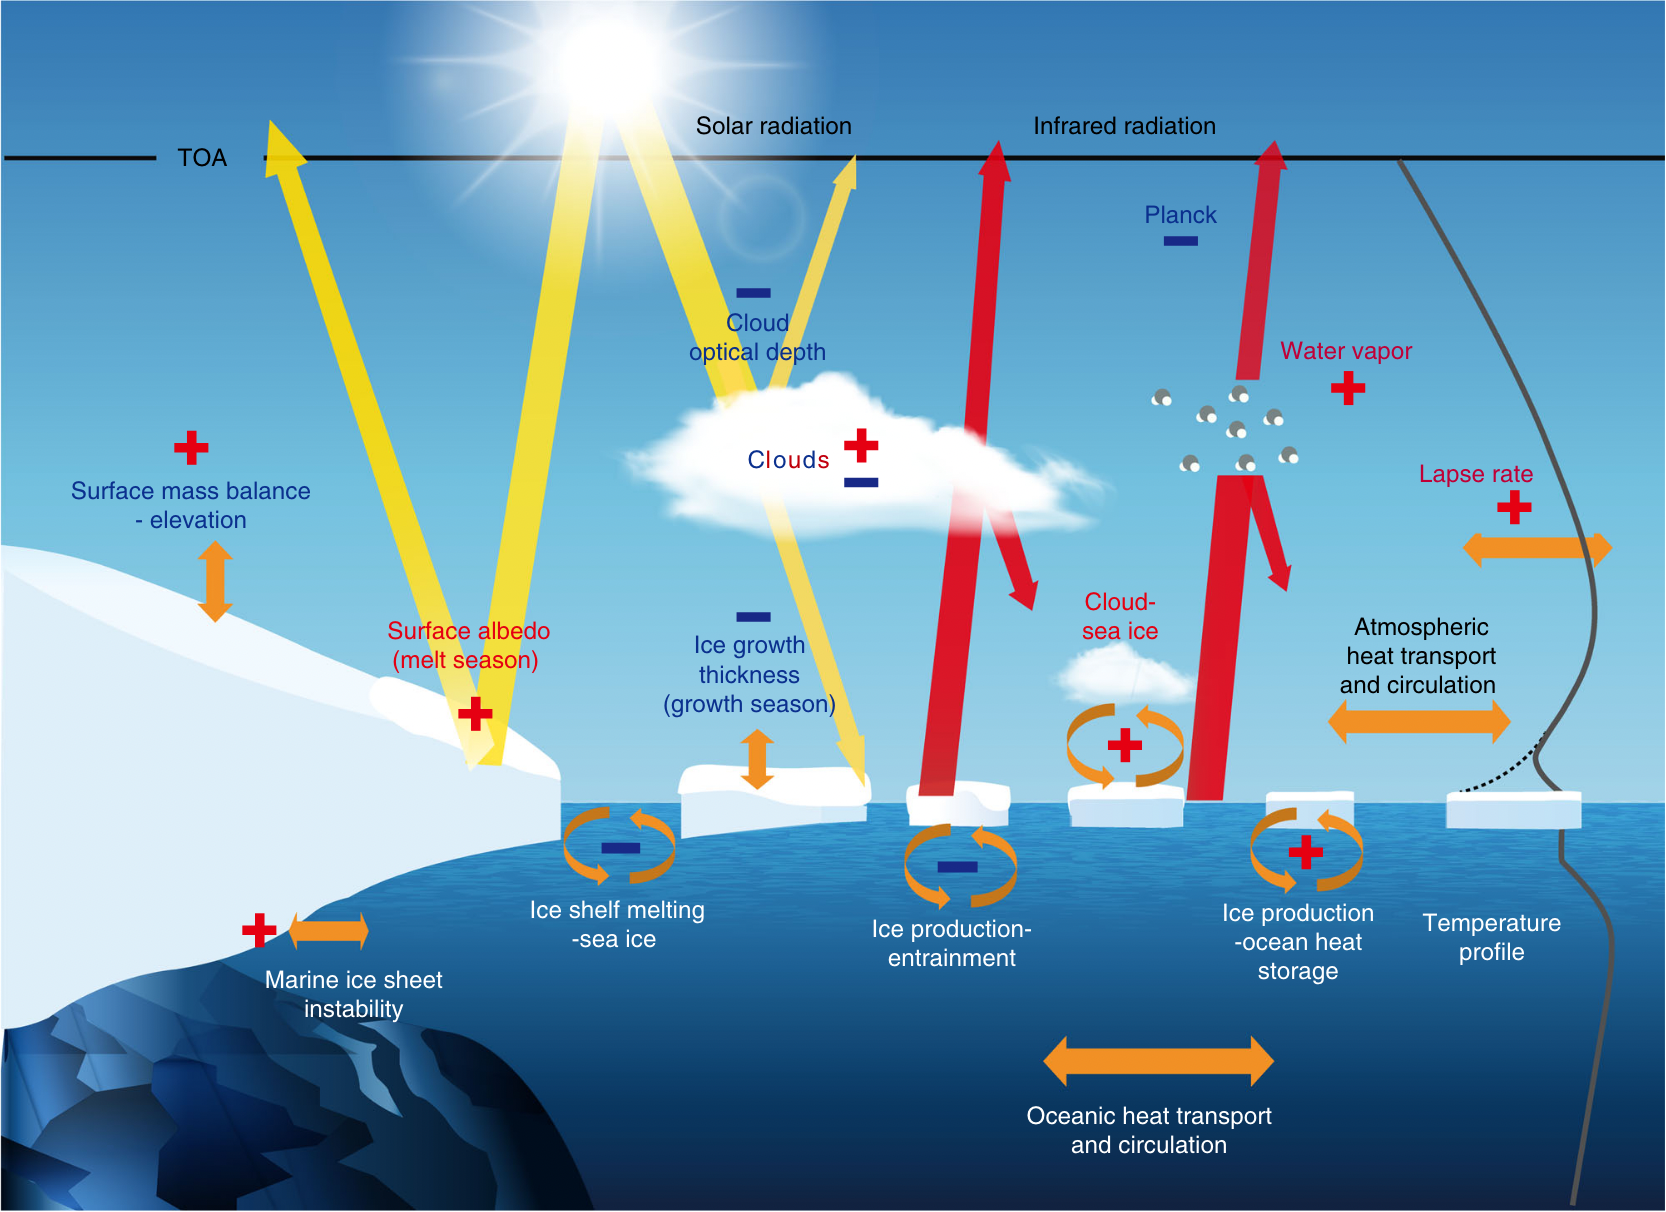
\includegraphics[width=80mm]{\sect/Goosse2018_1.png}
    \vspace{-4mm}
    \caption{A schematic of some important feedbacks in polar regions involving  the atmosphere, the ocean, sea ice and ice sheets.  
    Solar radiation (in yellow) and Infrared Radiation (in red) represent the shortwave (solar) and longwave (infrared) radiation exchanges. 
    Net effect due to clouds is unknown (therefor \(+/-\)). 
    The gray line on the right - simplified temperature profile in polar regions for the atmosphere and the ocean, the dashed line corresponding to a strong surface inversion. 
    Oceanic and atmospheric heat transport are mentioned but without signs as the processes involved are not restricted to polar regions and it is not clear if they could be formally expressed using a closed feedback loop.}
    \label{f:Goosse2018_1}
\end{figure}
\begin{figure}[ht]
    \centering
    \vspace{-4mm}
    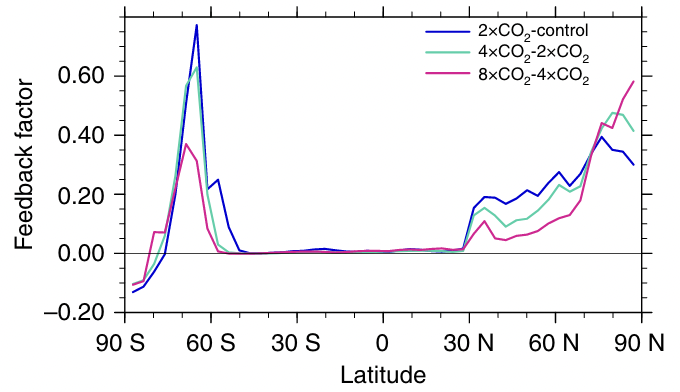
\includegraphics[width=80mm]{\sect/Goosse2018_2.png}
    \vspace{-4mm}
    \caption{Nonlinearity in the surface albedo feedback factor for three consecutive doublings of CO2. The feedback factor, defined as the ratio of the magnitude of the albedo feedback on the Planck feedback, is calculated using the radiative kernel technique and zonal averages are plotted for three consecutive doublings of CO2 concentrations in CCSM3. The global average feedback factor decreases from 0.097 for $2xCO2–CNTL$ to 0.053 for $8xCO2–4xCO2$}
    \label{f:Goosse2018_2}
\end{figure}
\begin{figure}[ht]
    \centering
    \vspace{-4mm}
    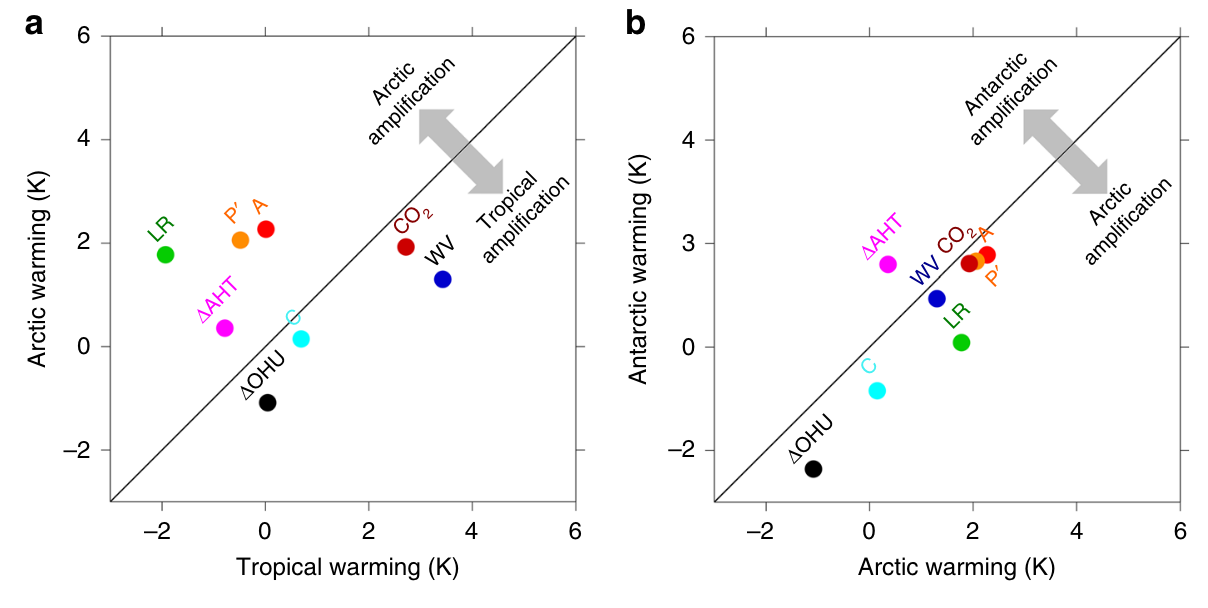
\includegraphics[width=80mm]{\sect/Goosse2018_3.png}
    \vspace{-4mm}
    \caption{Contributions of each feedback and atmospheric forcing to polar amplification. a Arctic (60–90N) relative to tropics \ (30S–30N), and b Antarctic (60-90S) relative to Arctic at year 100 of abrupt CO2 quadrupling in climate models involved in the fifth phase of the Coupled Model Intercomparison Project (CMIP5). 
    The feedbacks shown are the lapse rate (LR), surface albedo (A), water vapor (WV), cloud (C), and latitudinal variation in the Planck response (P’, local difference from its global-mean value \(\lambda \theta \)); the additional energetic contributions shown are the CO2 forcing (CO2), atmospheric heat transport convergence $( \delta AHT )$ and ocean heat uptake $( \delta OHT )$. 
    The feedbacks are expressed as warming contributions to the total temperature change}
    \label{f:Goosse2018_3}
\end{figure}
\subsection*{Questions and Comments}
\begin{itemize}
\item The structure functions of various orders seem highly applicable to studying turbulence (as has been done many times before) \cref{f:Goosse2018_1} shows the value of using a structure function instead of data or spectra. 
The structure function extracts the general shape of the data (the integral of the data) but smooths fluctuations and avoids the many frequencies in spectra. These might be useful inputs into PCA!
\end{itemize}
\newpage
\clearpage
\newpage
\clearpage




\def \sect {naakka2019}
\section{\citeauthor{\sect} \citeyear{\sect}}
\textbf{\citefield{\sect}{title}\nocite{\sect}}
\subsection*{Summary}
Horizontal atmospheric moisture transport distributes water vapour through the Arctic, and this has an impact on the radiative and hydrological conditions. Using ERA-I moisture transport between Arctic and mid latitudes is looked at. Meriodonal transport is not the only factor, with near surface transport being balanced between northward and southward transport. Total moisture transport (abs(north) + abs(south)) has a larger seasonal variability than net transport (mean meridional transport). Strenght of transport is related to atmospheric humidity over wind field. 
\subsection*{Important Figures}
\begin{figure}[ht]
    \centering
    \vspace{-4mm}
    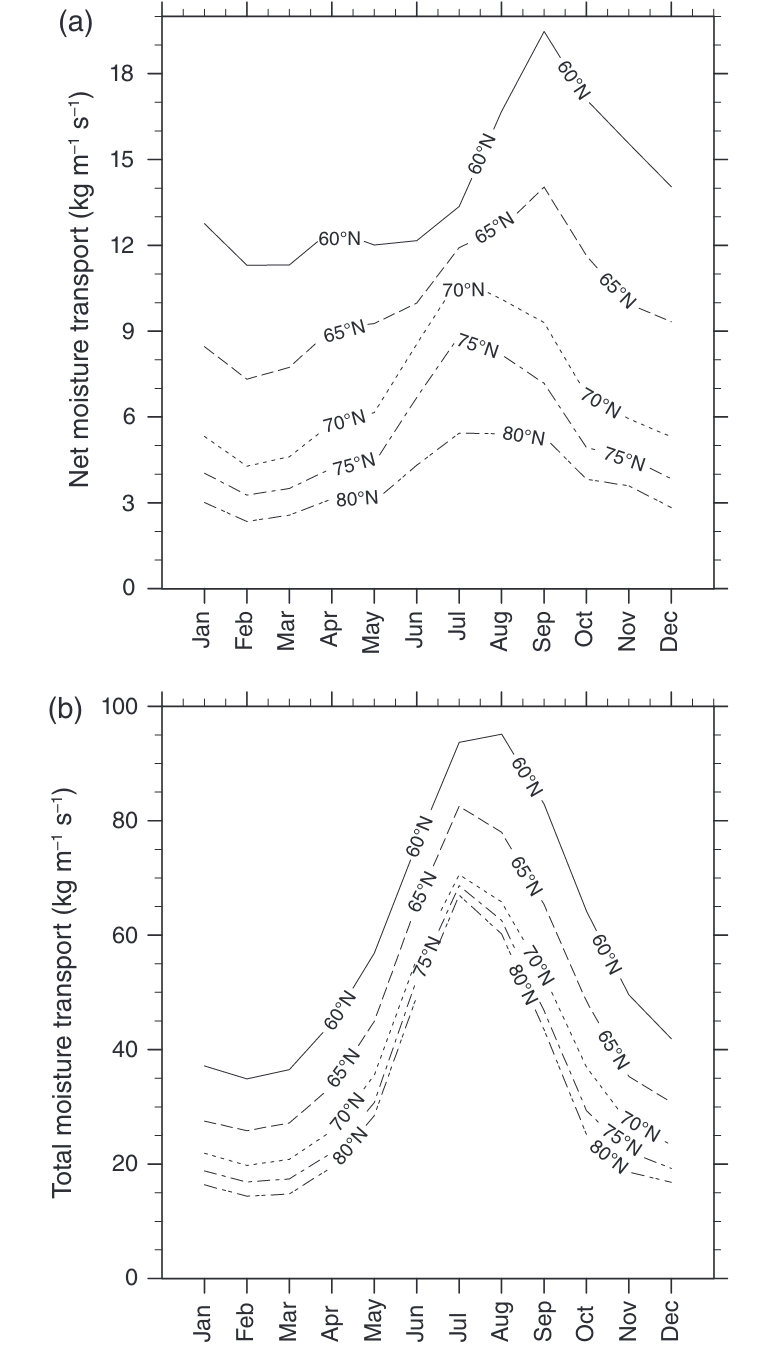
\includegraphics[width=80mm]{\sect/naakka2019_1.png}
    \vspace{-4mm}
    \caption{Vertically integrated surface (300 hPa) monthly mean meridional net moisture transport and total moisture transport. Total transport is the amount related to the seasonal cycle of atmopsheric moisture content and wind speed. Net transport is affected by the dynamical setting (cyclonic activity and large scale circulation patterns) and the humidity gradient between the Arctic and the lower latitudes. }\label{f:naakka2019_1.png}
\end{figure}
\begin{figure}[ht]
    \centering
    \vspace{-4mm}
    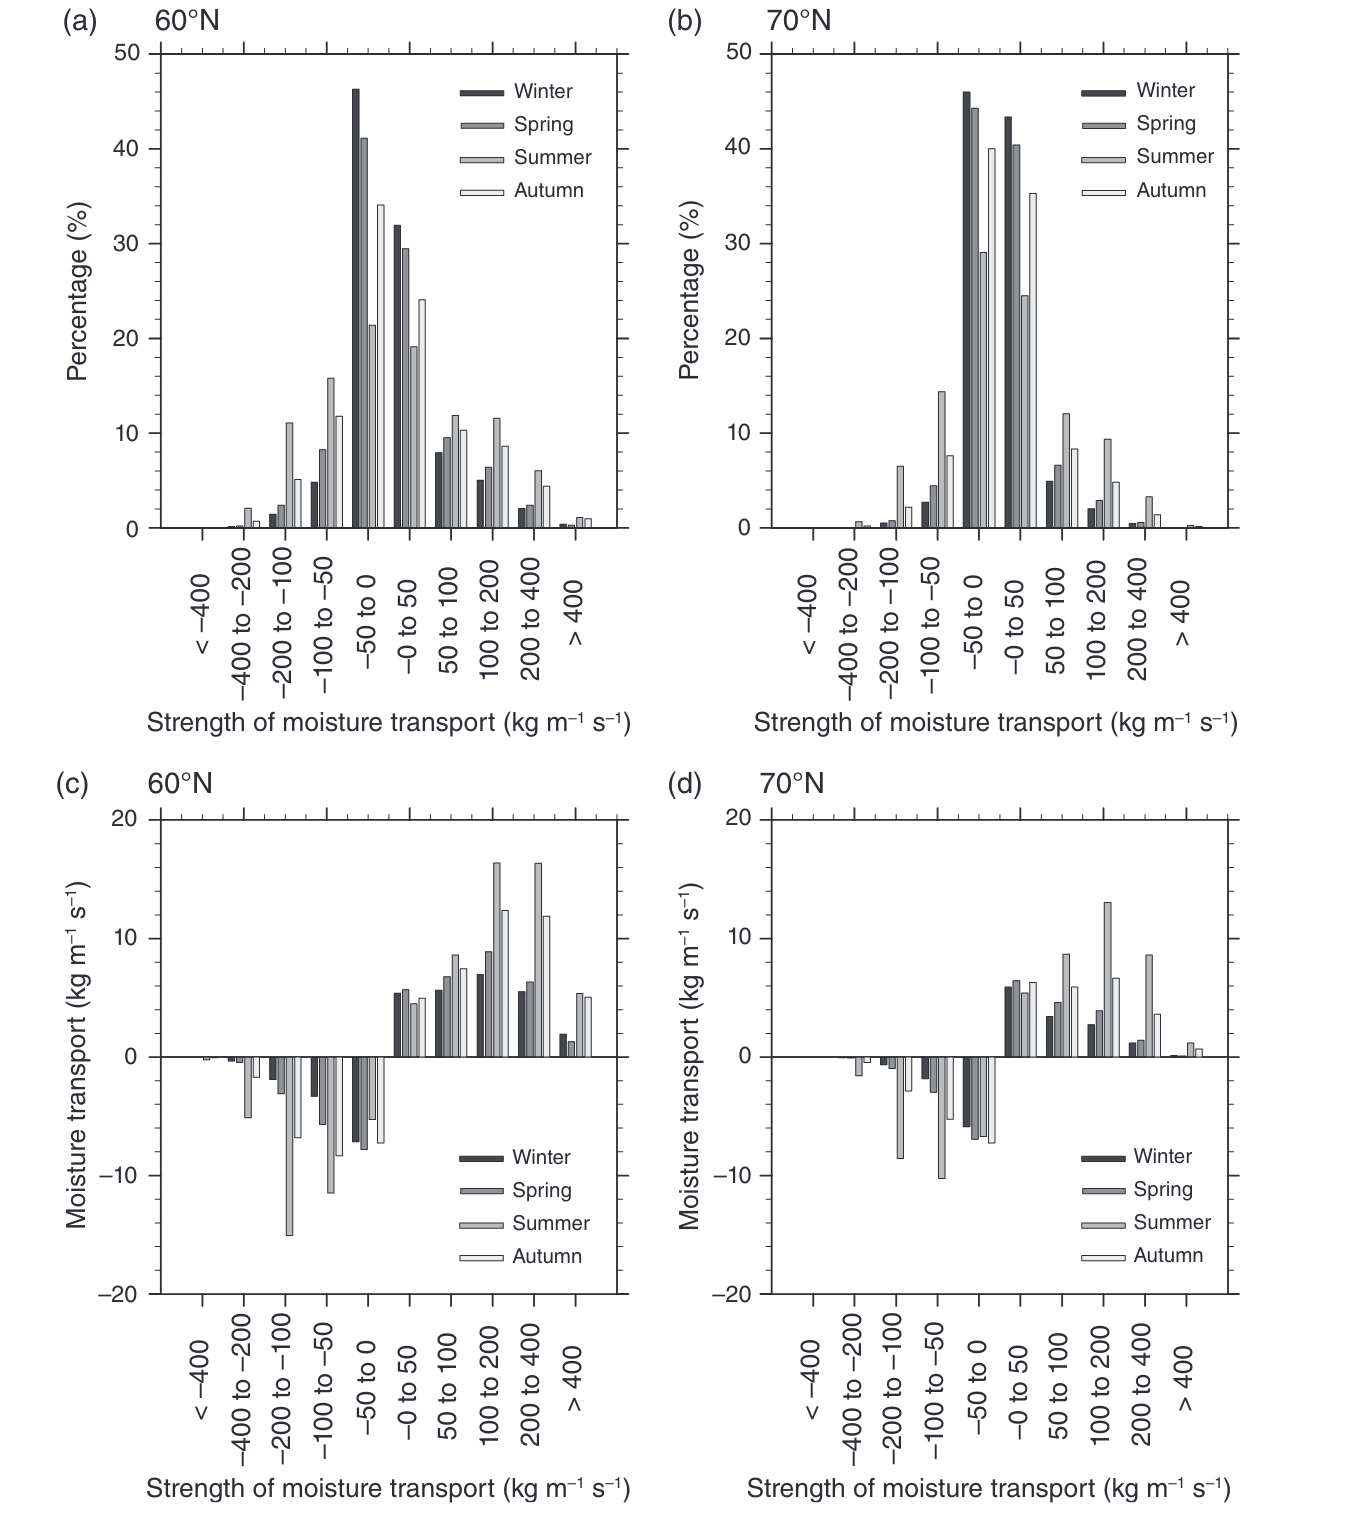
\includegraphics[width=80mm]{\sect/naakka2019_2.png}
    \vspace{-4mm}
    \caption{Strength of transport shown as frequency distributions of moisture transport strength computed from grid point values. Figures a and b show the occurence (VI meridional transport strength at 60° and 70° - weak for most of the time 
    ) and c and d (contribution of each moisture transport strength interval to meridional net moisture transport at 60° and 70°. See events of very strong north and south transports 
    ) show the contribution of these events. 60°N, northwards moisture transports with a magnitude $>$ 200 kg/m/s - responsible for 29\% of northwards moisture transport in winter their relative frequency of occurrence was only 3\%60°N, northwards moisture transports with a magnitude  200 kg kg/m/s - responsible for 42\% of northwards moisture transport in summer their relative frequency of occurrence was only 7\%}\label{f:naakka2019_2.png}
\end{figure}
\begin{figure}[ht]
    \centering
    \vspace{-4mm}
    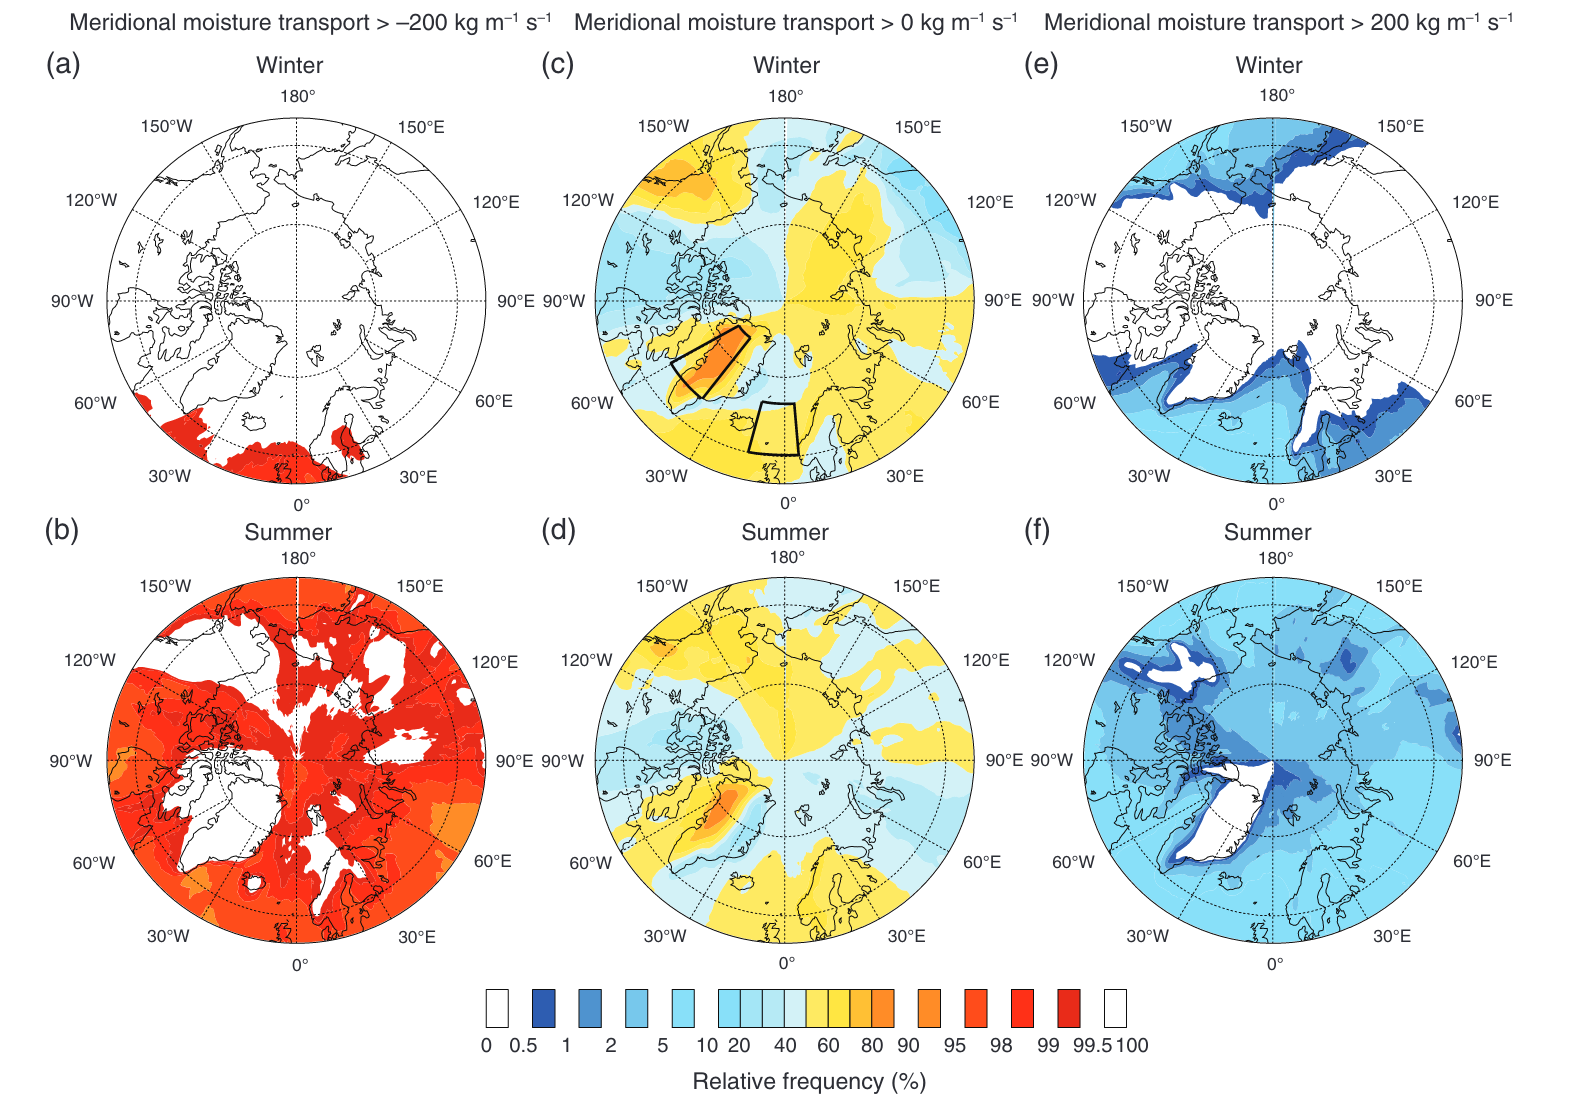
\includegraphics[width=80mm]{\sect/naakka2019_3.png}
    \vspace{-4mm}
    \caption{Frequencies of the amount of transport, which differ between seasons. 4a - Southwards moisture transports with $>$200 almost most absent in winter. 4b,f - wide area of big events Southwards and Northwards - due to higher specific humidity at this time. 4e - Winter - very intense transports ($>$200) over Atlantic and Pacific. Particularly for the WCA region, the summer has a high frequency of southward events of more than 200 kg/m/s. For transport north between 0 and 200, the WCA has a low frequency in the winter with a higher frequency in summer. Events ($>$200) are almost absent in winter, with a low frequency in summer. The most permanent southwards moisture flux was located in Northern Canada, where also the strongest net southwards moisture transport occurred.
     }\label{f:naakka2019_3.png}
\end{figure}
\begin{figure}[ht]
    \centering
    \vspace{-4mm}
    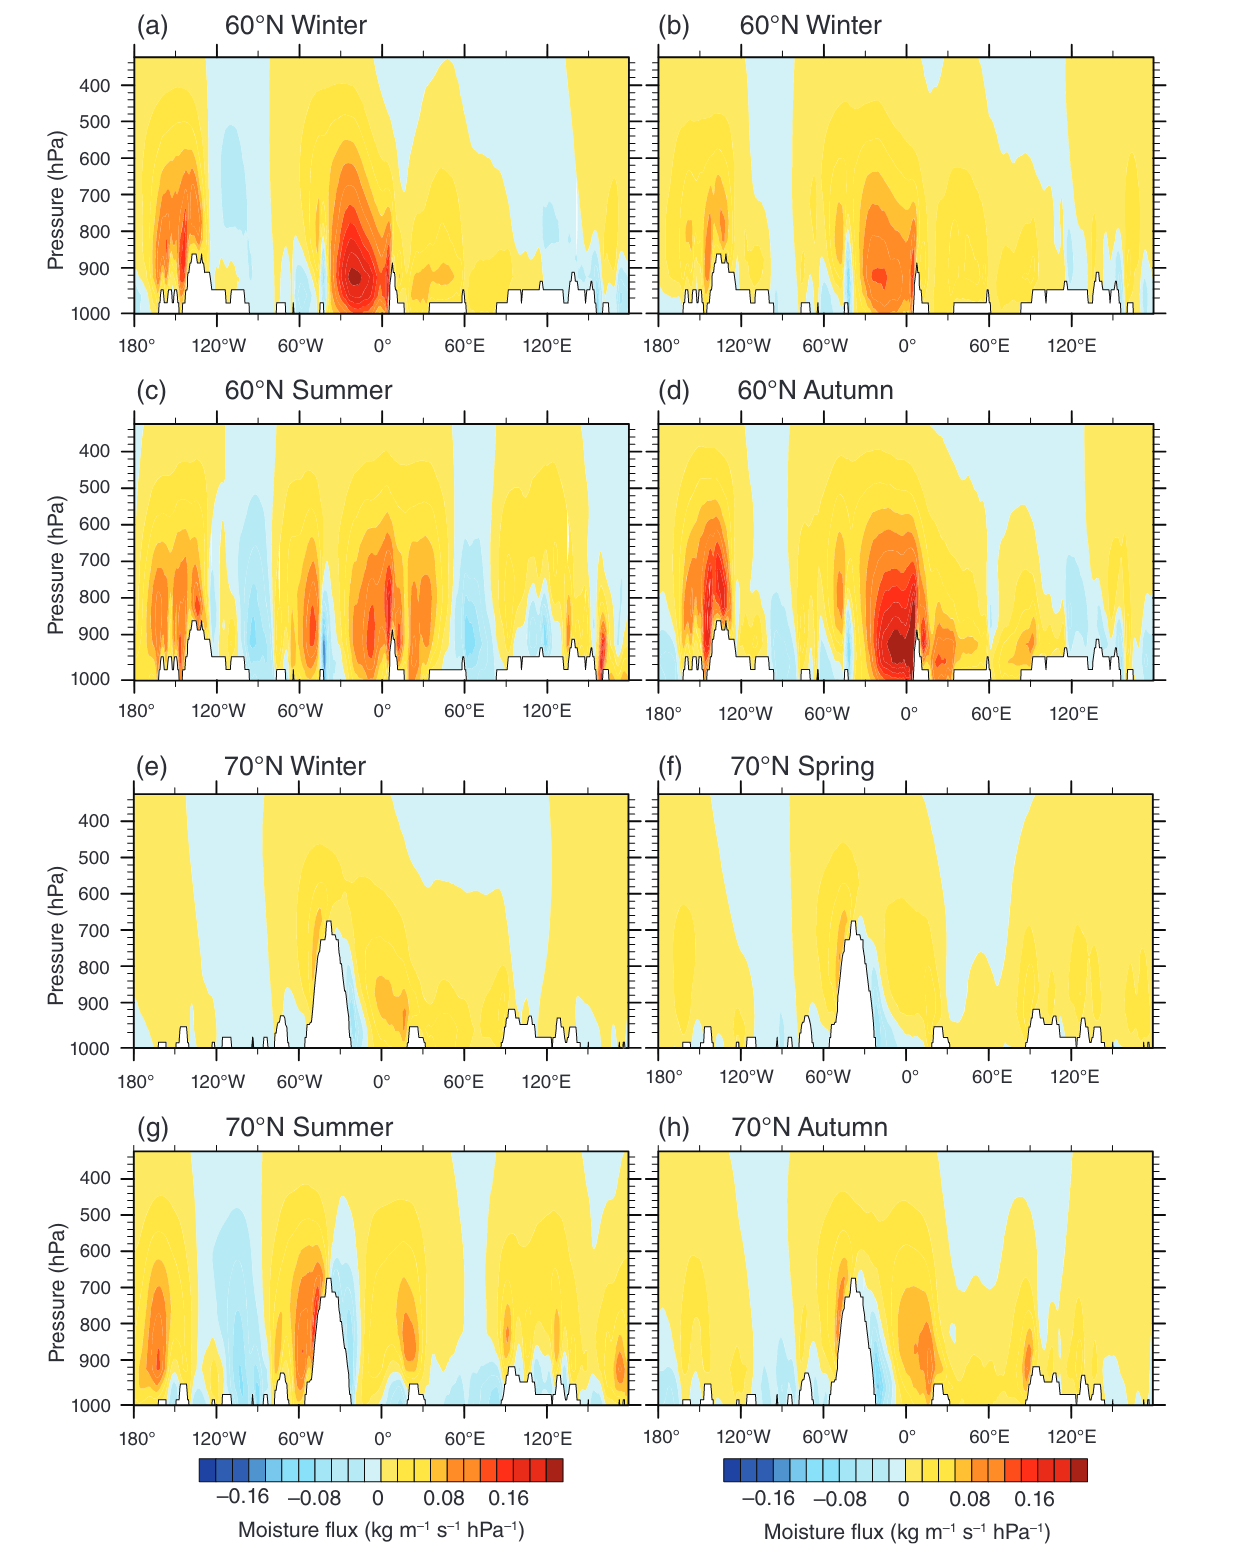
\includegraphics[width=80mm]{\sect/naakka2019_4.png}
    \vspace{-4mm}
    \caption{Looking at the cross section of seasonal mean, an increase in transport in the summer months over the continents is seen, with evaporation causing strengthening of the southwards moisture transport. There are longitudal variations in maximums. }\label{f:naakka2019_3.png}
\end{figure}
\subsection*{Questions and Comments}
A detailed look into moisture transport, which shows that the meridional net moisture transport at 60° to 70°N peaks at 100hPa higher than the northwards and southwards moisture transports.
Strong individual events contribute to a large part of the northwards moisture transport 
This is consistent with the result that the net moisture transport is generated by temporal variations of moisture fluxes. 
The seasonal cycle of the net moisture transport is related to the seasonal cycle of transient eddy moisture transport  and inter-annual variations of the net moisture transport - influenced by the stationary eddy moisture transport.
\newpage
\clearpage
\newpage
\clearpage




\def \sect {Hartmann2016}
\section{\citeauthor{\sect} \citeyear{\sect}}
\textbf{\citefield{\sect}{title}\nocite{\sect}}
\subsection*{Summary}
\subsubsection*{Chapter 1 - Introduction to the climate system}
\paragraph*{Atmospheric Temperature}
Global average temperature is 15°C. The lapse rate is the decline of temperature with height;
\begin{equation}
    \Gamma \equiv - \frac{\partial T}{\partial z} 
\end{equation}
the global mean tropospheric lapse rate is $6.5 K km^{-1}$
\begin{figure}[ht]
    \centering
    \vspace{-4mm}
    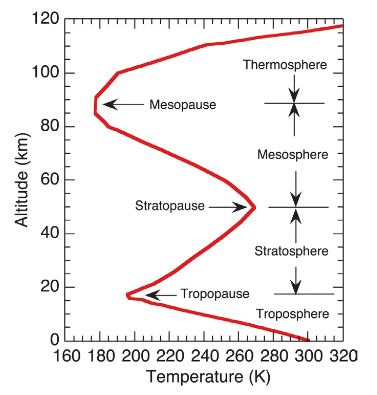
\includegraphics[width=80mm]{\sect/Hartmann2016_1.png}
    \vspace{-4mm}
    \caption{Main zones of atmosphere, atmosphere at 15°N for mean annual conditions.}\label{f:Hartmann2016_1}
\end{figure}
% or use eqnarray for equations
\subsection*{Important Figures}
\subsection*{Questions and Comments}
\newpage
\clearpage
\newpage
\clearpage




%sample for new entry 
\def \sect {Ali2020}
\section{\citeauthor{\sect} \citeyear{\sect}}
\textbf{\citefield{\sect}{title}\nocite{\sect}}
\subsection*{Summary}
Experiments ran in the Beaufort Gye. Two types of cloud states -> cloudy state of the boundary layer associated with a marine air mass origin -> clear state is tied to a continental air mass source

Through Lagrangian methods - created the first direct observational evidence of air mass transformations creating the cloudy and clear states of the Arctic boundary layer

\subsubsection*{Introduction}
MI - moist intrusions - can trigger cloud formation and surface warming - especially in winter 

No local moisture sources in winter 

Most of the warm air advected into the Arctic in winter is from MIs
Cloudy state of Arctic winter boundary layer - linked to advection of moist air masses

Direct observations of transformation from moist mid lat to dry Arctic air - lacking

\begin{itemize}
\item \textbf{Mechanism }
\item  Radiative cooling -> sensitive to moisture content of clouds
\item Warm air masses advected polewards rapid cooling = clouds
\item Liquid water clouds - radiatively opaque - strongest cooling at the cloud top
\item Cloud top cooling = turbulent mixing
\item Further cloud cooling = ice particles = mixed phase clouds (see in cloudy state)
\item Eventually - all liquid water lost by phase change and precip - ice cloud radiatvely transparent = surface cooling = surface based inversion layer - clear state 

Weather and climate models struggle to represent the transformation in lagrangian (follow the particle) framework 
= substantial energy biases 
Modelling air mass transitions - understand local microphysic of clouds and boundary layer turbulence 
Observations - Eulerian 
\end{itemize}
%\subsection*{Important Figures}
\subsection*{Questions and Comments}
This paper is useful as it uses back trajectory analysis to show where air masses originate from on specific days with specific events 
\newpage
\clearpage
\newpage
\clearpage




%sample for new entry 
\def \sect {Pithan2014}
\section{\citeauthor{\sect} \citeyear{\sect}}
\textbf{\citefield{\sect}{title}\nocite{\sect}}
\subsection*{Summary}
Cloud microphyics in Arctic regions.

Temperature inversions are important to understand due to their overall impact on local climate. They are formed from Arctic air masses which result in cloudy and clear states. Most climate models lack a representation of the cloudy state. SCM shows that bias is linked to inadequate mixed-phase cloud microphysics in cloudy state, and turbulent and conductive heat fluxes in the clear state


\begin{itemize}
\item Stronger warming at the surface than in the middle and upper troposphere leads to a positive lapse-rate feedback in the Arctic.
\item Temperature inversions occur when the air near the ground is colder than the air above it.
\item Low-level mixed-phase clouds play a key role in setting the surface fluxes and inversion strength, and many models struggle to represent these clouds at low temperatures.
\item The formation of inversions result in clear and cloudy conditions.
\item \textbf{Cloudy state}
\item Cooled liquid water is present
\item Very little surface radiative cooling occurs
\item Inversions -> elevated and relatively weak
\item \textbf{Clear state}
\item Surface radiative cooling ->  strong surface-based temperature inversions
\end{itemize}
\subsection*{Important Figures}
\subsection*{Questions and Comments}
\newpage
\clearpage
\newpage
\clearpage


%sample for new entry 
\def \sect {Hartmann2016}
\section{\citeauthor{\sect} \citeyear{\sect}}
\textbf{\citefield{\sect}{title}\nocite{\sect}}
\subsection*{Summary}
Global physical climate 
\subsection*{Important Figures}
\subsection*{Questions and Comments}
\newpage
\clearpage
\newpage
\clearpage



\printbibliography
% \bibliographystyle{apalike}
% \bibliography{prop}

\end{document}
